\documentclass[12pt]{article}

\usepackage[top=5em, bottom=5em, left=5em, right=5em]{geometry}
\usepackage{tikz}
\usetikzlibrary{positioning}

\setlength\parindent{0em}
\setlength\parskip{1em}

\title {Assignment 3}

\author {Hendrik Werner s4549775}

\begin{document}
\maketitle

This was done in collaboration with Constantin Blach (s4329872).

\section{} %1
Initial state:

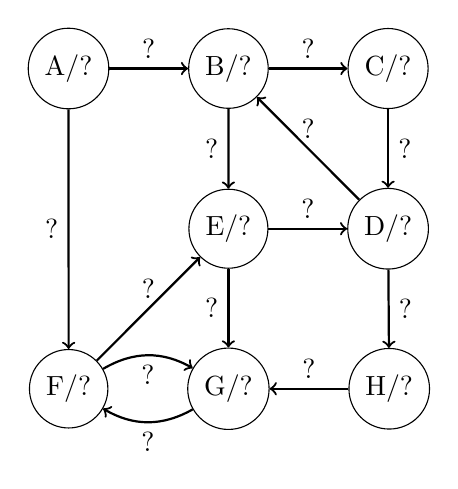
\begin{tikzpicture}[c/.style={circle, draw}]
	\node [c] (A) {A/?};
	\node [c, right=of A] (B) {B/?};
	\node [c, right=of B] (C) {C/?};
	\node [c, below=of C] (D) {D/?};
	\node [c, left =of D] (E) {E/?};
	\node [c, below=of E] (G) {G/?};
	\node [c, left =of G] (F) {F/?};
	\node [c, right=of G] (H) {H/?};

	\path[->, thick] (A) edge node [above] {?} (B);
	\path[->, thick] (A) edge node [left ] {?} (F);
	\path[->, thick] (B) edge node [above] {?} (C);
	\path[->, thick] (B) edge node [left ] {?} (E);
	\path[->, thick] (C) edge node [right] {?} (D);
	\path[->, thick] (D) edge node [above] {?} (B);
	\path[->, thick] (D) edge node [right] {?} (H);
	\path[->, thick] (E) edge node [above] {?} (D);
	\path[->, thick] (E) edge node [left ] {?} (G);
	\path[->, thick] (F) edge node [above] {?} (E);
	\path[->, thick] (F) edge [bend left] node [below] {?} (G);
	\path[->, thick] (G) edge [bend left] node [below] {?} (F);
	\path[->, thick] (H) edge node [above] {?} (G);
\end{tikzpicture}

\begin{enumerate}
	\item
	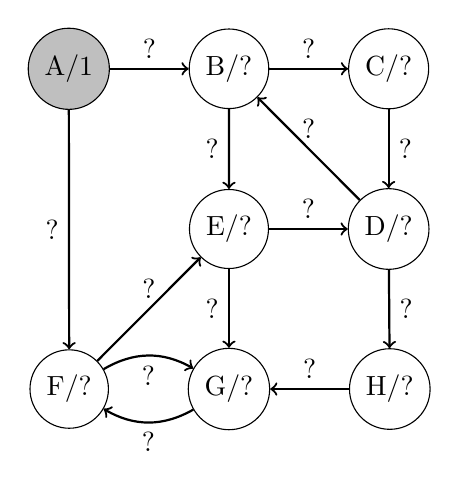
\begin{tikzpicture}[baseline=(A.north), c/.style={circle, draw}, visited/.style={fill=lightgray}]
		\node [c, visited] (A) {A/1};
		\node [c, right=of A] (B) {B/?};
		\node [c, right=of B] (C) {C/?};
		\node [c, below=of C] (D) {D/?};
		\node [c, left =of D] (E) {E/?};
		\node [c, below=of E] (G) {G/?};
		\node [c, left =of G] (F) {F/?};
		\node [c, right=of G] (H) {H/?};

		\path[->, thick] (A) edge node [above] {?} (B);
		\path[->, thick] (A) edge node [left ] {?} (F);
		\path[->, thick] (B) edge node [above] {?} (C);
		\path[->, thick] (B) edge node [left ] {?} (E);
		\path[->, thick] (C) edge node [right] {?} (D);
		\path[->, thick] (D) edge node [above] {?} (B);
		\path[->, thick] (D) edge node [right] {?} (H);
		\path[->, thick] (E) edge node [above] {?} (D);
		\path[->, thick] (E) edge node [left ] {?} (G);
		\path[->, thick] (F) edge node [above] {?} (E);
		\path[->, thick] (F) edge [bend left] node [below] {?} (G);
		\path[->, thick] (G) edge [bend left] node [below] {?} (F);
		\path[->, thick] (H) edge node [above] {?} (G);
	\end{tikzpicture}

	\item
	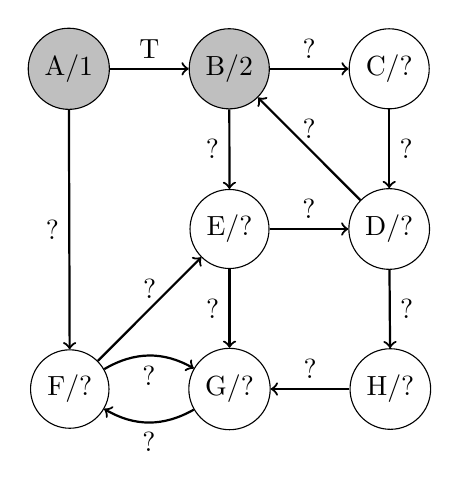
\begin{tikzpicture}[baseline=(A.north), c/.style={circle, draw}, visited/.style={fill=lightgray}]
		\node [c, visited] (A) {A/1};
		\node [c, visited, right=of A] (B) {B/2};
		\node [c, right=of B] (C) {C/?};
		\node [c, below=of C] (D) {D/?};
		\node [c, left =of D] (E) {E/?};
		\node [c, below=of E] (G) {G/?};
		\node [c, left =of G] (F) {F/?};
		\node [c, right=of G] (H) {H/?};

		\path[->, thick] (A) edge node [above] {T} (B);
		\path[->, thick] (A) edge node [left ] {?} (F);
		\path[->, thick] (B) edge node [above] {?} (C);
		\path[->, thick] (B) edge node [left ] {?} (E);
		\path[->, thick] (C) edge node [right] {?} (D);
		\path[->, thick] (D) edge node [above] {?} (B);
		\path[->, thick] (D) edge node [right] {?} (H);
		\path[->, thick] (E) edge node [above] {?} (D);
		\path[->, thick] (E) edge node [left ] {?} (G);
		\path[->, thick] (F) edge node [above] {?} (E);
		\path[->, thick] (F) edge [bend left] node [below] {?} (G);
		\path[->, thick] (G) edge [bend left] node [below] {?} (F);
		\path[->, thick] (H) edge node [above] {?} (G);
	\end{tikzpicture}

	\item
	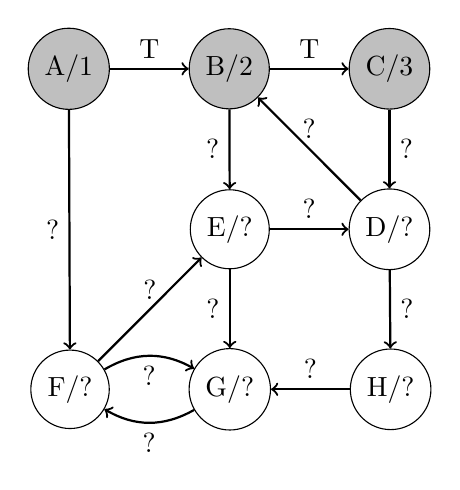
\begin{tikzpicture}[baseline=(A.north), c/.style={circle, draw}, visited/.style={fill=lightgray}]
		\node [c, visited] (A) {A/1};
		\node [c, visited, right=of A] (B) {B/2};
		\node [c, visited, right=of B] (C) {C/3};
		\node [c, below=of C] (D) {D/?};
		\node [c, left =of D] (E) {E/?};
		\node [c, below=of E] (G) {G/?};
		\node [c, left =of G] (F) {F/?};
		\node [c, right=of G] (H) {H/?};

		\path[->, thick] (A) edge node [above] {T} (B);
		\path[->, thick] (A) edge node [left ] {?} (F);
		\path[->, thick] (B) edge node [above] {T} (C);
		\path[->, thick] (B) edge node [left ] {?} (E);
		\path[->, thick] (C) edge node [right] {?} (D);
		\path[->, thick] (D) edge node [above] {?} (B);
		\path[->, thick] (D) edge node [right] {?} (H);
		\path[->, thick] (E) edge node [above] {?} (D);
		\path[->, thick] (E) edge node [left ] {?} (G);
		\path[->, thick] (F) edge node [above] {?} (E);
		\path[->, thick] (F) edge [bend left] node [below] {?} (G);
		\path[->, thick] (G) edge [bend left] node [below] {?} (F);
		\path[->, thick] (H) edge node [above] {?} (G);
	\end{tikzpicture}

	\item
	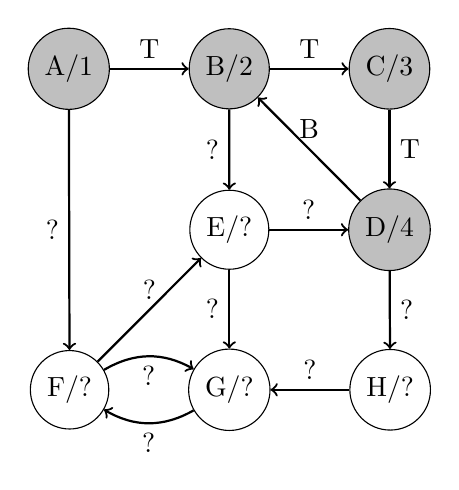
\begin{tikzpicture}[baseline=(A.north), c/.style={circle, draw}, visited/.style={fill=lightgray}]
		\node [c, visited] (A) {A/1};
		\node [c, visited, right=of A] (B) {B/2};
		\node [c, visited, right=of B] (C) {C/3};
		\node [c, visited, below=of C] (D) {D/4};
		\node [c, left =of D] (E) {E/?};
		\node [c, below=of E] (G) {G/?};
		\node [c, left =of G] (F) {F/?};
		\node [c, right=of G] (H) {H/?};

		\path[->, thick] (A) edge node [above] {T} (B);
		\path[->, thick] (A) edge node [left ] {?} (F);
		\path[->, thick] (B) edge node [above] {T} (C);
		\path[->, thick] (B) edge node [left ] {?} (E);
		\path[->, thick] (C) edge node [right] {T} (D);
		\path[->, thick] (D) edge node [above] {B} (B);
		\path[->, thick] (D) edge node [right] {?} (H);
		\path[->, thick] (E) edge node [above] {?} (D);
		\path[->, thick] (E) edge node [left ] {?} (G);
		\path[->, thick] (F) edge node [above] {?} (E);
		\path[->, thick] (F) edge [bend left] node [below] {?} (G);
		\path[->, thick] (G) edge [bend left] node [below] {?} (F);
		\path[->, thick] (H) edge node [above] {?} (G);
	\end{tikzpicture}

	\item
	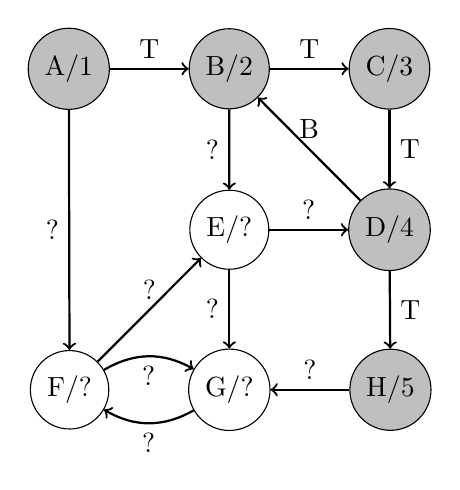
\begin{tikzpicture}[baseline=(A.north), c/.style={circle, draw}, visited/.style={fill=lightgray}]
		\node [c, visited] (A) {A/1};
		\node [c, visited, right=of A] (B) {B/2};
		\node [c, visited, right=of B] (C) {C/3};
		\node [c, visited, below=of C] (D) {D/4};
		\node [c, left =of D] (E) {E/?};
		\node [c, below=of E] (G) {G/?};
		\node [c, left =of G] (F) {F/?};
		\node [c, visited, right=of G] (H) {H/5};

		\path[->, thick] (A) edge node [above] {T} (B);
		\path[->, thick] (A) edge node [left ] {?} (F);
		\path[->, thick] (B) edge node [above] {T} (C);
		\path[->, thick] (B) edge node [left ] {?} (E);
		\path[->, thick] (C) edge node [right] {T} (D);
		\path[->, thick] (D) edge node [above] {B} (B);
		\path[->, thick] (D) edge node [right] {T} (H);
		\path[->, thick] (E) edge node [above] {?} (D);
		\path[->, thick] (E) edge node [left ] {?} (G);
		\path[->, thick] (F) edge node [above] {?} (E);
		\path[->, thick] (F) edge [bend left] node [below] {?} (G);
		\path[->, thick] (G) edge [bend left] node [below] {?} (F);
		\path[->, thick] (H) edge node [above] {?} (G);
	\end{tikzpicture}

	\item
	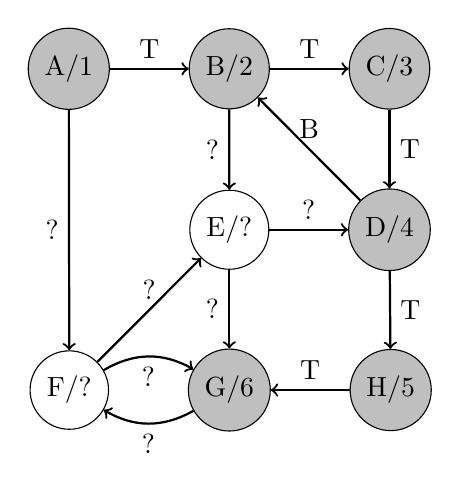
\begin{tikzpicture}[baseline=(A.north), c/.style={circle, draw}, visited/.style={fill=lightgray}]
		\node [c, visited] (A) {A/1};
		\node [c, visited, right=of A] (B) {B/2};
		\node [c, visited, right=of B] (C) {C/3};
		\node [c, visited, below=of C] (D) {D/4};
		\node [c, left =of D] (E) {E/?};
		\node [c, visited, below=of E] (G) {G/6};
		\node [c, left =of G] (F) {F/?};
		\node [c, visited, right=of G] (H) {H/5};

		\path[->, thick] (A) edge node [above] {T} (B);
		\path[->, thick] (A) edge node [left ] {?} (F);
		\path[->, thick] (B) edge node [above] {T} (C);
		\path[->, thick] (B) edge node [left ] {?} (E);
		\path[->, thick] (C) edge node [right] {T} (D);
		\path[->, thick] (D) edge node [above] {B} (B);
		\path[->, thick] (D) edge node [right] {T} (H);
		\path[->, thick] (E) edge node [above] {?} (D);
		\path[->, thick] (E) edge node [left ] {?} (G);
		\path[->, thick] (F) edge node [above] {?} (E);
		\path[->, thick] (F) edge [bend left] node [below] {?} (G);
		\path[->, thick] (G) edge [bend left] node [below] {?} (F);
		\path[->, thick] (H) edge node [above] {T} (G);
	\end{tikzpicture}

	\item
	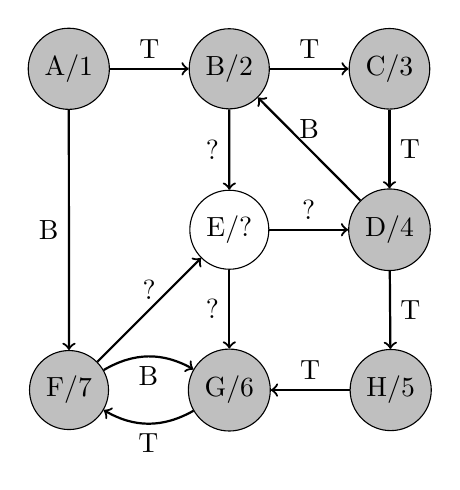
\begin{tikzpicture}[baseline=(A.north), c/.style={circle, draw}, visited/.style={fill=lightgray}]
		\node [c, visited] (A) {A/1};
		\node [c, visited, right=of A] (B) {B/2};
		\node [c, visited, right=of B] (C) {C/3};
		\node [c, visited, below=of C] (D) {D/4};
		\node [c, left =of D] (E) {E/?};
		\node [c, visited, below=of E] (G) {G/6};
		\node [c, visited, left =of G] (F) {F/7};
		\node [c, visited, right=of G] (H) {H/5};

		\path[->, thick] (A) edge node [above] {T} (B);
		\path[->, thick] (A) edge node [left ] {B} (F);
		\path[->, thick] (B) edge node [above] {T} (C);
		\path[->, thick] (B) edge node [left ] {?} (E);
		\path[->, thick] (C) edge node [right] {T} (D);
		\path[->, thick] (D) edge node [above] {B} (B);
		\path[->, thick] (D) edge node [right] {T} (H);
		\path[->, thick] (E) edge node [above] {?} (D);
		\path[->, thick] (E) edge node [left ] {?} (G);
		\path[->, thick] (F) edge node [above] {?} (E);
		\path[->, thick] (F) edge [bend left] node [below] {B} (G);
		\path[->, thick] (G) edge [bend left] node [below] {T} (F);
		\path[->, thick] (H) edge node [above] {T} (G);
	\end{tikzpicture}

	\item
	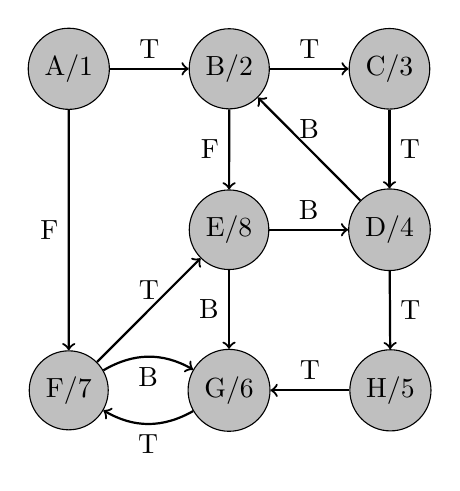
\begin{tikzpicture}[baseline=(A.north), c/.style={circle, draw}, visited/.style={fill=lightgray}]
		\node [c, visited] (A) {A/1};
		\node [c, visited, right=of A] (B) {B/2};
		\node [c, visited, right=of B] (C) {C/3};
		\node [c, visited, below=of C] (D) {D/4};
		\node [c, visited, left =of D] (E) {E/8};
		\node [c, visited, below=of E] (G) {G/6};
		\node [c, visited, left =of G] (F) {F/7};
		\node [c, visited, right=of G] (H) {H/5};

		\path[->, thick] (A) edge node [above] {T} (B);
		\path[->, thick] (A) edge node [left ] {F} (F);
		\path[->, thick] (B) edge node [above] {T} (C);
		\path[->, thick] (B) edge node [left ] {F} (E);
		\path[->, thick] (C) edge node [right] {T} (D);
		\path[->, thick] (D) edge node [above] {B} (B);
		\path[->, thick] (D) edge node [right] {T} (H);
		\path[->, thick] (E) edge node [above] {B} (D);
		\path[->, thick] (E) edge node [left ] {B} (G);
		\path[->, thick] (F) edge node [above] {T} (E);
		\path[->, thick] (F) edge [bend left] node [below] {B} (G);
		\path[->, thick] (G) edge [bend left] node [below] {T} (F);
		\path[->, thick] (H) edge node [above] {T} (G);
	\end{tikzpicture}
\end{enumerate}

\section{} %2
You can find the minimum number of semesters necessary by using a kind of reverse BFS.

\begin{enumerate}
	\item Initialize the semester counter to 1.
	\item Mark nodes with out-degree 0 (the final courses) as visited.
	\item \label{loop} Follow the ingoing edges of the last visited nodes and mark their origin nodes as visited when all of their outgoing edges connect to visited nodes.
	\item Increment the semester counter.
	\item If any of these nodes have an in-degree $> 0$, go to \ref{loop}, else go to \ref{end}
	\item \label{end} Return the semester counter.
\end{enumerate}

Example:

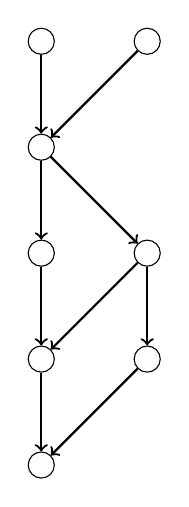
\begin{tikzpicture}[c/.style={circle, draw}, v/.style={fill=gray}]
	\node[c] (a) {};
	\node[c, right=of a] (b) {};
	\node[c, below=of a] (c) {};
	\node[c, below=of c] (d) {};
	\node[c, right=of d] (e) {};
	\node[c, below=of d] (f) {};
	\node[c, below=of e] (g) {};
	\node[c, below=of f] (h) {};

	\path[->, thick] (a) edge (c);
	\path[->, thick] (b) edge (c);
	\path[->, thick] (c) edge (d);
	\path[->, thick] (c) edge (e);
	\path[->, thick] (d) edge (f);
	\path[->, thick] (e) edge (f);
	\path[->, thick] (e) edge (g);
	\path[->, thick] (f) edge (h);
	\path[->, thick] (g) edge (h);
\end{tikzpicture}

\begin{enumerate}
	\item
	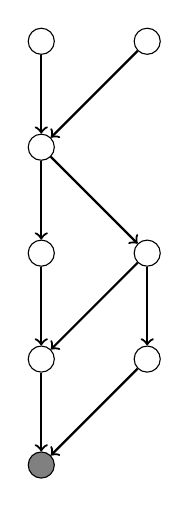
\begin{tikzpicture}[baseline=(a.south), c/.style={circle, draw}, v/.style={fill=gray}]
		\node[c] (a) {};
		\node[c, right=of a] (b) {};
		\node[c, below=of a] (c) {};
		\node[c, below=of c] (d) {};
		\node[c, right=of d] (e) {};
		\node[c, below=of d] (f) {};
		\node[c, below=of e] (g) {};
		\node[c, v, below=of f] (h) {};

		\path[->, thick] (a) edge (c);
		\path[->, thick] (b) edge (c);
		\path[->, thick] (c) edge (d);
		\path[->, thick] (c) edge (e);
		\path[->, thick] (d) edge (f);
		\path[->, thick] (e) edge (f);
		\path[->, thick] (e) edge (g);
		\path[->, thick] (f) edge (h);
		\path[->, thick] (g) edge (h);
	\end{tikzpicture}
	Semester counter = 1

	\item
	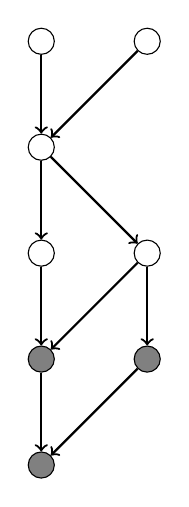
\begin{tikzpicture}[baseline=(a.south), c/.style={circle, draw}, v/.style={fill=gray}]
		\node[c] (a) {};
		\node[c, right=of a] (b) {};
		\node[c, below=of a] (c) {};
		\node[c, below=of c] (d) {};
		\node[c, right=of d] (e) {};
		\node[c, v, below=of d] (f) {};
		\node[c, v, below=of e] (g) {};
		\node[c, v, below=of f] (h) {};

		\path[->, thick] (a) edge (c);
		\path[->, thick] (b) edge (c);
		\path[->, thick] (c) edge (d);
		\path[->, thick] (c) edge (e);
		\path[->, thick] (d) edge (f);
		\path[->, thick] (e) edge (f);
		\path[->, thick] (e) edge (g);
		\path[->, thick] (f) edge (h);
		\path[->, thick] (g) edge (h);
	\end{tikzpicture}
	Semester counter = 2

	\item
	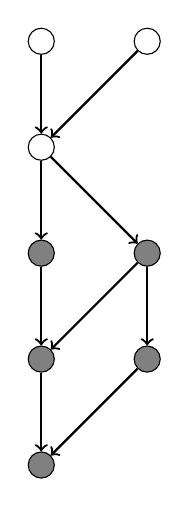
\begin{tikzpicture}[baseline=(a.south), c/.style={circle, draw}, v/.style={fill=gray}]
		\node[c] (a) {};
		\node[c, right=of a] (b) {};
		\node[c, below=of a] (c) {};
		\node[c, v, below=of c] (d) {};
		\node[c, v, right=of d] (e) {};
		\node[c, v, below=of d] (f) {};
		\node[c, v, below=of e] (g) {};
		\node[c, v, below=of f] (h) {};

		\path[->, thick] (a) edge (c);
		\path[->, thick] (b) edge (c);
		\path[->, thick] (c) edge (d);
		\path[->, thick] (c) edge (e);
		\path[->, thick] (d) edge (f);
		\path[->, thick] (e) edge (f);
		\path[->, thick] (e) edge (g);
		\path[->, thick] (f) edge (h);
		\path[->, thick] (g) edge (h);
	\end{tikzpicture}
	Semester counter = 3

	\item
	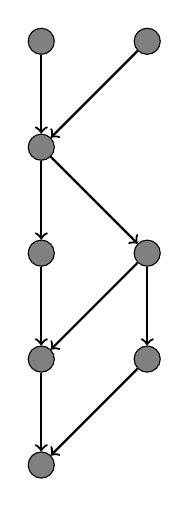
\begin{tikzpicture}[baseline=(a.south), c/.style={circle, draw}, v/.style={fill=gray}]
		\node[c, v] (a) {};
		\node[c, v, right=of a] (b) {};
		\node[c, v, below=of a] (c) {};
		\node[c, v, below=of c] (d) {};
		\node[c, v, right=of d] (e) {};
		\node[c, v, below=of d] (f) {};
		\node[c, v, below=of e] (g) {};
		\node[c, v, below=of f] (h) {};

		\path[->, thick] (a) edge (c);
		\path[->, thick] (b) edge (c);
		\path[->, thick] (c) edge (d);
		\path[->, thick] (c) edge (e);
		\path[->, thick] (d) edge (f);
		\path[->, thick] (e) edge (f);
		\path[->, thick] (e) edge (g);
		\path[->, thick] (f) edge (h);
		\path[->, thick] (g) edge (h);
	\end{tikzpicture}
	Semester counter = 5
\end{enumerate}

You need at least 5 semesters to take all courses in this example.

\section{} %3
\section{} %4
\section{} %5
\section{} %6

\end{document}
